
%!TEX root = thesis.tex

\chapter{Background}\label{chpt:background}

In this chapter, we discuss some background knowledge and previous work helpful to understanding the rest of the dissertation. 
Broadly speaking, we will make use of inference techniques for probabilistic modeling, collaborative filtering method for recommender systems, and causal inference. We give a high-level overview of the three fields and introduce some necessary definitions that will be used in the subsequent chapters. 

\section{Probabilistic modeling and inference techniques}\label{chpt:background:sec:inference}

We begin by defining the general problem setup for probabilistic latent variable models. We observe data $\mbx = \{x_1, \dots, x_N\}$. We assume the data is generated stochastically by a model $p(\mbx \g \mbz, \theta)$ that is governed by some latent variables $\mbz = \{z_1, \dots, z_N\}$ as well as model parameters $\mb\theta$\footnote{The distinction between latent variables $\mbz$ and model parameters $\mb\theta$ can be somewhat arbitrary. Here we follow the convention that the dimensionality of the latent variables grows with the number of observations (hence both $\mbx$ and $\mbz$ are indexed by $n$), while that of model parameters does not. Latent variables and model parameters loosely correspond to \textit{local variables} and \textit{global variables} in \citet{hoffman2013stochastic}}. We can also incorporate priors $p(\mbz, \mb\theta)$. We leave the dependency structure of prior generic. This class of models covers a wide range of commonly used models, to name a few: mixture models, hidden Markov models, probabilistic matrix factorization \citep{salakhutdinov2008probabilistic}, and mixed-membership models (e.g., latent Dirichlet allocation \citep{blei2003latent}, and stochastic blockmodels \citep{DBLP:journals/jmlr/AiroldiBFX08}).

\Cref{chpt:background:fig:general} demonstrates the graphical model representation for the general latent variable models described above. Shaded nodes represent observed variables. Unshaded nodes represent
hidden (unobserved) variables. A directed edge from node $a$ to node $b$
denotes that the variable $b$ depends on the value of variable
$a$. Plates denote replication by the value in the lower corner
of the plate. We use doted line to indicate that the dependency between model parameters $\mb\theta$ and latent variables $\mbz$ are optional -- it depends on how the prior $p(\mbz, \mb\theta)$ is specified. 

\begin{figure}[ht]
  \centering
     \begin{tikzpicture}

  % Define nodes
  \node[obs] 			(x) {$x_n$};
  \node[latent, above=.8cm of x] (z) {$z_n$};
  \node[latent, left=.6cm of z] (theta) {$\mb\theta$};

  % Connect the nodes
  \edge {z} {x} ; %
  \edge {theta} {x};
  \edge[densely dotted] {theta}{z};

  % Plates
  \plate {xz} {(x)(z)} {$N$};

\end{tikzpicture}


  \caption{Graphical model representation for the general latent variable models. Doted line is used to indicate that the dependency between model parameters $\mb\theta$ and latent variables $\mbz$ are optional -- it depends on how the prior $p(\mbz, \mb\theta)$ is specified. }
\label{chpt:background:fig:general}
\end{figure}

In Bayesian inference, the
goal is to reason about the posterior distribution over the model parameters and latent variables conditioned on the data, which is given by Bayes' rule:
\begin{equation}
p(\mb{\theta}, \mbz \g \mbx) = \frac{p(\mbx \g \mbz, \mb{\theta}) p(\mbz, \mb{\theta})}{ p(\mbx)} = \frac{p(\mbx \g \mbz, \mb{\theta}) p(\mbz, \mb{\theta})}{ \int_\mb{\theta} \int_\mbz p(\mbx \g \mbz, \mb{\theta}) p(\mbz, \mb{\theta}) \dif \mbz \dif \mb\theta}
\label{chpt:background:eq:bayes}
\end{equation}
Through posterior inference, we are able to uncover the latent structure induced by the model. Except in very simple models, posterior $p(\mb{\theta}, \mbz \g \mbx)$ is generally intractable to compute due to the normalizing constant $p(\mbx)$ which requires computing the integral in the denominator of \Cref{chpt:background:eq:bayes}. In practice, people normally resort to \gls{MCMC} methods \citep{neal1993probabilistic,robert2013monte} to obtain samples from the posterior distribution to form a Monte Carlo estimator about the predictive quantities. Despite the asymptotic guarantees, \gls{MCMC} methods are generally unable to analyze large-scale data. Scaling Bayesian inference to large-scale data is an active research area (see \citet{angelino2016patterns} for an extensive survey). In \Cref{chpt:background:sec:vi}, we will introduce variational inference, a scalable deterministic alternative to \gls{MCMC}. 

Alternatively, it is also possible (and computationally simpler) to only obtain a point estimate of the parameters of interest instead of reasoning about the entire posterior via maximum likelihood estimation (MLE) or maximum \textit{a posteriori} (MAP):

\begin{equation}
\mb\theta^\textrm{MLE} = \argmax_\mb\theta \log p(\mbx \g \mb\theta) = \argmax_\mb\theta \log \int_\mbz p(\mbx, \mbz \g \mb\theta) \dif\mbz
\label{chpt:background:eq:mle}
\end{equation}
\begin{equation}
\mb\theta^\textrm{MAP} = \argmax_\mb\theta \log p(\mb\theta, \mbz \g \mbx) = \argmax_\mb\theta \log \int_\mbz p(\mb\theta, \mbz, \mbx) \dif\mbz
\label{chpt:backgroun:eq:map}
\end{equation}

For models with latent variables, \gls{EM} \citep{dempster1977maximum} algorithm is usually required to obtain these point estimates, which we will turn to next. 

\subsection{Parameter estimation via expectation-maximization}\label{chpt:background:sec:em}

In this section, we introduce the \gls{EM} algorithm for parameter estimation. There exist different derivations of the algorithm in the literature. Here we choose to introduce it in the variational framework to highlight its close connection to variational inference, which we will introduce in the following section. We derive the \gls{EM} algorithm for maximum likelihood estimation (\Cref{chpt:background:eq:mle}) -- it only requires minor modification for maximum \textit{a posteriori} (\Cref{chpt:backgroun:eq:map}).

To obtain the maximum likelihood estimates, typically we write down the so-called \textit{observable data log-likelihood} $\log p(\mbx \g \mb\theta)$ and optimize it with respect to the model parameters $\mb\theta$. One of the problems with directly optimizing the observable data log-likelihood for models with latent variables $\mbz$ is that it requires to integrate over all the latent variables $\log \int_\mbz p(\mbx, \mbz \g \mb\theta) \dif\mbz$, which is generally intractable. As a workaround, we instead optimize the \textit{complete data log-likelihood} $\log p(\mbx, \mbz \g \mb \theta)$ by introducing a \textit{variational distribution} $q(\mbz)$ and applying Jensen's inequality:
\begin{equation}
\begin{split}
\log p(\mbx \g \mb\theta) &= \log\int_\mbz p(\mbx, \mbz \g \mb\theta) \dif{\mbz}\\
&= \log\int_\mbz q(\mbz) \frac{p(\mbx, \mbz \g \mb\theta)}{q(\mbz)} \dif{\mbz}\\
&\geq \int_\mbz q(\mbz) \log\frac{p(\mbx, \mbz \g \mb\theta)}{q(\mbz)} \dif\mbz\\
&= \EE{q}{\log p(\mbx, \mbz \g \mb\theta)} - \EE{q}{\log q(\mbz)}.
\end{split}
\label{chpt:background:eq:em}
\end{equation}
We obtain a lower bound of the log-likelihood $\log p(\mbx \g \mb\theta)$ that we are interested in optimizing. The tightness of this bound depends on the variational distribution $q(\mbz)$. We could of course find out the optimal $q(\mbz)$ by exploring when the equality holds for Jensen's inequality. However, we will solve it from a different angle here. We first explore the slack by applying Jensen's inequality:
\begin{equation}
\begin{split}
\Delta =& \log p(\mbx \g \mb\theta) - \int_\mbz q(\mbz) \log\frac{p(\mbx, \mbz \g \mb\theta)}{q(\mbz)} \dif\mbz \\
=& \int_\mbz q(\mbz)\log p(\mbx \g \mb\theta) - \int_\mbz q(\mbz) \log\frac{p(\mbx, \mbz \g \mb\theta)}{q(\mbz)} \dif\mbz\\
=& \int_\mbz q(\mbz) \log\frac{p(\mbx \g \mb\theta) q(\mbz)} {p(\mbx, \mbz \g \mb\theta)}\dif\mbz\\
=& \int_\mbz q(\mbz) \log\frac{ q(\mbz)} {p(\mbz \g \mbx, \mb\theta)}\dif\mbz \equiv \textrm{KL}(q_\mbz\|p_{\mbz \g \mbx, \mb\theta})
\end{split}
\label{chpt:background:eq:em_kl}
\end{equation}
Thus, the difference is the \gls{KL} divergence between the variational distribution $q(\mbz)$ and the posterior distribution $p(\mbz \g \mbx, \mb\theta)$. We can re-write the log-likelihood as:
\[
\log p(\mbx \g \mb\theta) = \underbrace{\EE{q}{\log p(\mbx, \mbz \g \mb\theta)} - \EE{q}{\log q(\mbz)}}_{\cL(q, \mb\theta)} + \textrm{KL}(q_\mbz\|p_{\mbz \g \mbx, \mb\theta}).
\]
Since the \gls{KL}-divergence $\textrm{KL}(q_\mbz\|p_{\mbz \g \mbx, \mb\theta})$ is non-negative and equals $0$ only if $q(\mbz) = p(\mbz \g \mbx, \mb\theta)$, $a.s.$, $\cL(q, \mb\theta)$ acts as a tight lower-bound that equals $\log p(\mbx \g \mb\theta)$ when we set $q(\mbz)$ to $p(\mbz \g \mbx, \mb\theta)$. \gls{EM} algorithm optimizes $\cL(q, \mb\theta)$ by iteratively applying the following E(xpectation) and M(aximization) steps:

\parhead{E-step:} By setting $q(\mbz) = p(\mbz \g \mbx, \mb\theta)$, we obtain the optimal variational distribution, closing the gap between log-likelihood $\log p(\mbx \g \mb\theta)$ and the lower bound $\cL(q, \mb\theta)$. 

\parhead{M-step:} We have $q(\mbz)$ fixed from E-step and optimize $\cL(q, \mb\theta)$ with respect to the model parameters $\mb\theta$, which is equivalent to the following:
\begin{equation*}
\mb\theta^\new = \argmax_\mb\theta \EE{q}{\log p(\mbx, \mbz \g \mb\theta)},
\end{equation*}
since $\EE{q}{\log q(\mbz)}$ does not depend on $\mb\theta$.\footnote{In principle, $\mb\theta^\new$ does not have to fully optimize the objective $\EE{q}{\log p(\mbx, \mbz, \g \mb\theta)}$, as long as the new values increase it (e.g., by taking a few gradient steps). This is referred as generalized \gls{EM} \citep{neal1998view}.} Unless we have reached a stationary point, the lower bound $\cL(q, \mb\theta)$ will increase with the new parameters $\mb\theta^\new$. The new parameters $\mb\theta^\new$ will also make the \gls{KL}-divergence $\textrm{KL}(q_\mbz\|p_{\mbz \g \mbx, \mb\theta})$ greater than $0$, which creates gap between the log-likelihood and $\cL(q, \mb{\theta})$. This gap will be closed in the next E-step. Chapter 9 of \citet{Bishop:2006:PRM:1162264} provides a clear illustrative demonstration of the \gls{EM} algorithm.  

\gls{EM} algorithm is a typical example of \textit{coordinate ascent} \citep{bertsekas1999nonlinear}, where in each E- and M-step, we fix one of the variables of interest---$\mb\theta$ in E-step and $q(\mbz)$ in M-step---and optimize with respect to the other one.


\subsection{Variational inference}\label{chpt:background:sec:vi}

Variational inference is a deterministic alternative to \gls{MCMC} methods \citep{jordan1999introduction,wainwright2008graphical,blei2016variational}. In Bayesian inference, we aim to reason about the posterior $p(\mbz, \mb\theta \g \mbx)$ which is almost always intractable to compute. The basic idea behind variational inference is to choose a tractable family of variational distributions $q(\mbz, \mb\theta)$ to approximate the intractable posterior $p(\mbz, \theta | \mbx)$, so that the \gls{KL}-divergence between the variational distribution and the true posterior $\textrm{KL}(q_{\mbz, \mb\theta}\|p_{\mbz, \mb\theta \g \mbx})$ is minimized.

Variational inference turns the problem of Bayesian inference into a one of  optimization, which enables us to leverage the advances from optimization community, e.g., by making use of stochastic optimization, we can scale variational inference to massive dataset \citep{hoffman2013stochastic}.

To utilize variational inference for approximate Bayesian inference, we introduce the variational distribution $q(\mbz, \mb\theta)$ and lower bound the marginal likelihood, similar to \Cref{chpt:background:eq:em}:
\begin{equation}
\begin{split}
\log p(\mbx) &= \log\int_{\mbz, \mb\theta} p(\mbx, \mbz, \mb\theta) \dif{\mbz} \dif\mb\theta \\
&\geq \EE{q}{\log p(\mbx, \mbz, \mb\theta)} - \EE{q}{\log q(\mbz, \mb\theta)}\triangleq \cL.
\end{split}
\label{chpt:background:eq:vi}
\end{equation}
Here the model parameters $\mb\theta$ are treated the same as latent variables $\mbz$ with some pre-specified prior $p(\mbz, \mb\theta)$.\footnote{Variational inference can also be applied to the MLE/MAP case in \Cref{chpt:background:sec:em} where we only marginalize out latent variables $\mbz$ to obtain point estimates of model parameters $\mb\theta$. This happens in the E-step, when the posterior $p(\mbz \g \mbx, \mb\theta)$ is intractable to compute exactly, which leads to the variational \gls{EM} algorithm \citep{beal2003variational}.} $\cL$ is usually referred as \gls{ELBO}, since it is a lower bound of the model evidence $\log p(\mbx)$. Based on derivation similar to \Cref{chpt:background:eq:em_kl} (omitted for brevity), we can show that optimizing \gls{ELBO} is equivalent to minimizing the \gls{KL} divergence between the variational distribution $q(\mbz, \mb\theta)$ and the posterior of interest $p(\mbz, \mb\theta \g \mbx)$. Once we obtain the approximating posterior that minimizes the \gls{KL}-divergence, we can use it as a proxy of the true posterior to form prediction. 

So far we haven't specified how to select the variational distribution $q(\mbz, \mb\theta)$. One popular choice is the mean-field family which is completely factorized: $q(\mbz, \mb\theta) = \left(\prod_{d} q_d(z_{d})\right) \left(\prod_i q_i(\theta_i) \right)$. With mean-field family, we can obtain the general form for the optimal variational distributions:
\begin{equation}
\begin{split}
q^*_d(z_d) &\propto \exp\{\EE{q_{-d}}{\log p(z_d, \mbx, z_{-d}, \mb\theta)}\}
\\
q^*_i(\theta_i) &\propto \exp\{\EE{q_{-i}}{\log p(\theta_i, \mbx, \mbz, \theta_{-i})}\},
\end{split}
\label{chpt:background:eq:opt_q}
\end{equation}
where $z_{-d}$ is used to index all of $\mbz$ except the $d$th dimension, and $\EE{q_{-d}}{\cdot}$ denotes taking expectation with respect to everything except $q_d(z_d)$. ($\theta_{-i}$ and $\EE{q_{-i}}{\cdot}$ are similarly defined.)

For conditional conjugate model where the complete conditionals $p(z_d \g \mbx, z_{-d}, \mb\theta)$ and $p(\theta_i \g \mbx, \mbz, \theta_{-i})$ are in exponential family, the distributional form of \Cref{chpt:background:eq:opt_q} can be computed exactly. This leads to the standard coordinate ascent variational inference algorithm: we iteratively set $q_d(z_d)$ and $q_i(\theta_i)$ to its optimal form while keeping everything else fixed across the dimensions and repeat this procedure until convergence. 

\section{Recommender systems}\label{chpt:background:sec:recsys}

Making good recommendations is an important problem on the web. In the
recommendation problem, we observe how a set of users interacts with a
set of items, and our goal is to show each user a set of previously
unseen items that she will like.  Broadly speaking, recommender
systems use historical data to infer users' preferences, and then use
the inferred preferences to suggest items.  Good recommender
systems are essential as the web grows; users are overwhelmed with
choice.

\subsection{Explicit and implicit feedback} \label{chpt:background:sec:data}

Traditionally there are two modes of the recommendation problem: recommendation from explicit data and recommendation from implicit data.  With explicit
data, users rate some items (positively, negatively, or along a
spectrum) and we can predict their missing ratings (the task of \textit{rating prediction}, popularized by the Netflix Prize\footnote{\url{http://www.netflixprize.com/}}). This is called explicit data because users' preferences are expressed in an explicit fashion: positively rated items indicate types of items that they
like; negatively rated items indicate items that they do not like. For explicit data, it is enough to only use the rated items to infer a user's
preferences as we have both positive and negative examples. Explicit data is of great value, but it is often difficult to obtain. 

In implicit data, each user expresses a binary decision about items\footnote{In principle, implicit data can go beyond binary: For example, the number of times a user listened to certain songs can also be considered as implicit feedback. However, in practice we find that the binary indicator of \textit{interaction} tends to carry the most signal. }---for
example this can be clicking, purchasing, viewing---and we aim to
predict unclicked items that she would want to click on. (We use the verb ``click'' throughout this dissertation for concreteness; this can be any type of interaction, including
``download,'' ``purchase,'' ``listen,'' or ``watch.'') Unlike
ratings data, implicit data is easily accessible. While ratings data
requires action on the part of the users, implicit data is often a
natural byproduct of their behavior, e.g., browsing histories, click
logs, and past purchases. Despite the ease of access, implicit data is inherently noisy, as users' preferences are expressed through implicit actions and we only observe positive signals: we know users click on items they like, but we do not know why an item is unclicked. We will explore recommender systems for both implicit and explicit data in this dissertation in \Cref{chpt:expomf} and \Cref{chpt:causal_rec}, respectively.

\subsection{Collaborative filtering for recommender systems} \label{chpt:background:sec:cf}

Collaborative filtering is the workhorse of recommender systems. It is widely used in many commercial websites, e.g., Amazon uses various collaborative filtering algorithms to suggest products (``Customers Who Bought This Item Also Bought''), and Netflix uses collaborative filtering algorithms extensively in their homepage to suggest new movies and TV shows to watch.

Collaborative filtering analyzes user preferences for items by exploiting the similarity patterns across users. There are two major classes of collaborative filtering algorithms: neighborhood-based model \citep{sarwar2001item} and the matrix factorization model \citep{koren2009matrix}. In this dissertation, we will mainly focus on the matrix factorization for collaborative filtering. 

\subsubsection{Matrix factorization for collaborative filtering} 
\label{chpt:background:sec:mf_cf}

User-item preference data, whether explicit or implicit, can be encoded in a user by item matrix. Throughout this dissertation, a user is indexed by $u \in \{1, \dots, U\}$, an item is indexed by $i \in \{1, \dots, I\}$, and we will refer to this user by item matrix as the \emph{click matrix} or the \emph{interaction matrix}. Given the observed entries in this matrix $\{y_{ui}: (u, i) \in \cO\}$, the recommendation task is often framed as filling in the unobserved entries.  Matrix factorization models, which infer (latent) user preferences and item attributes by factorizing the click matrix, are standard in recommender systems \citep{koren2009matrix}. 

\begin{figure}
  \centering
    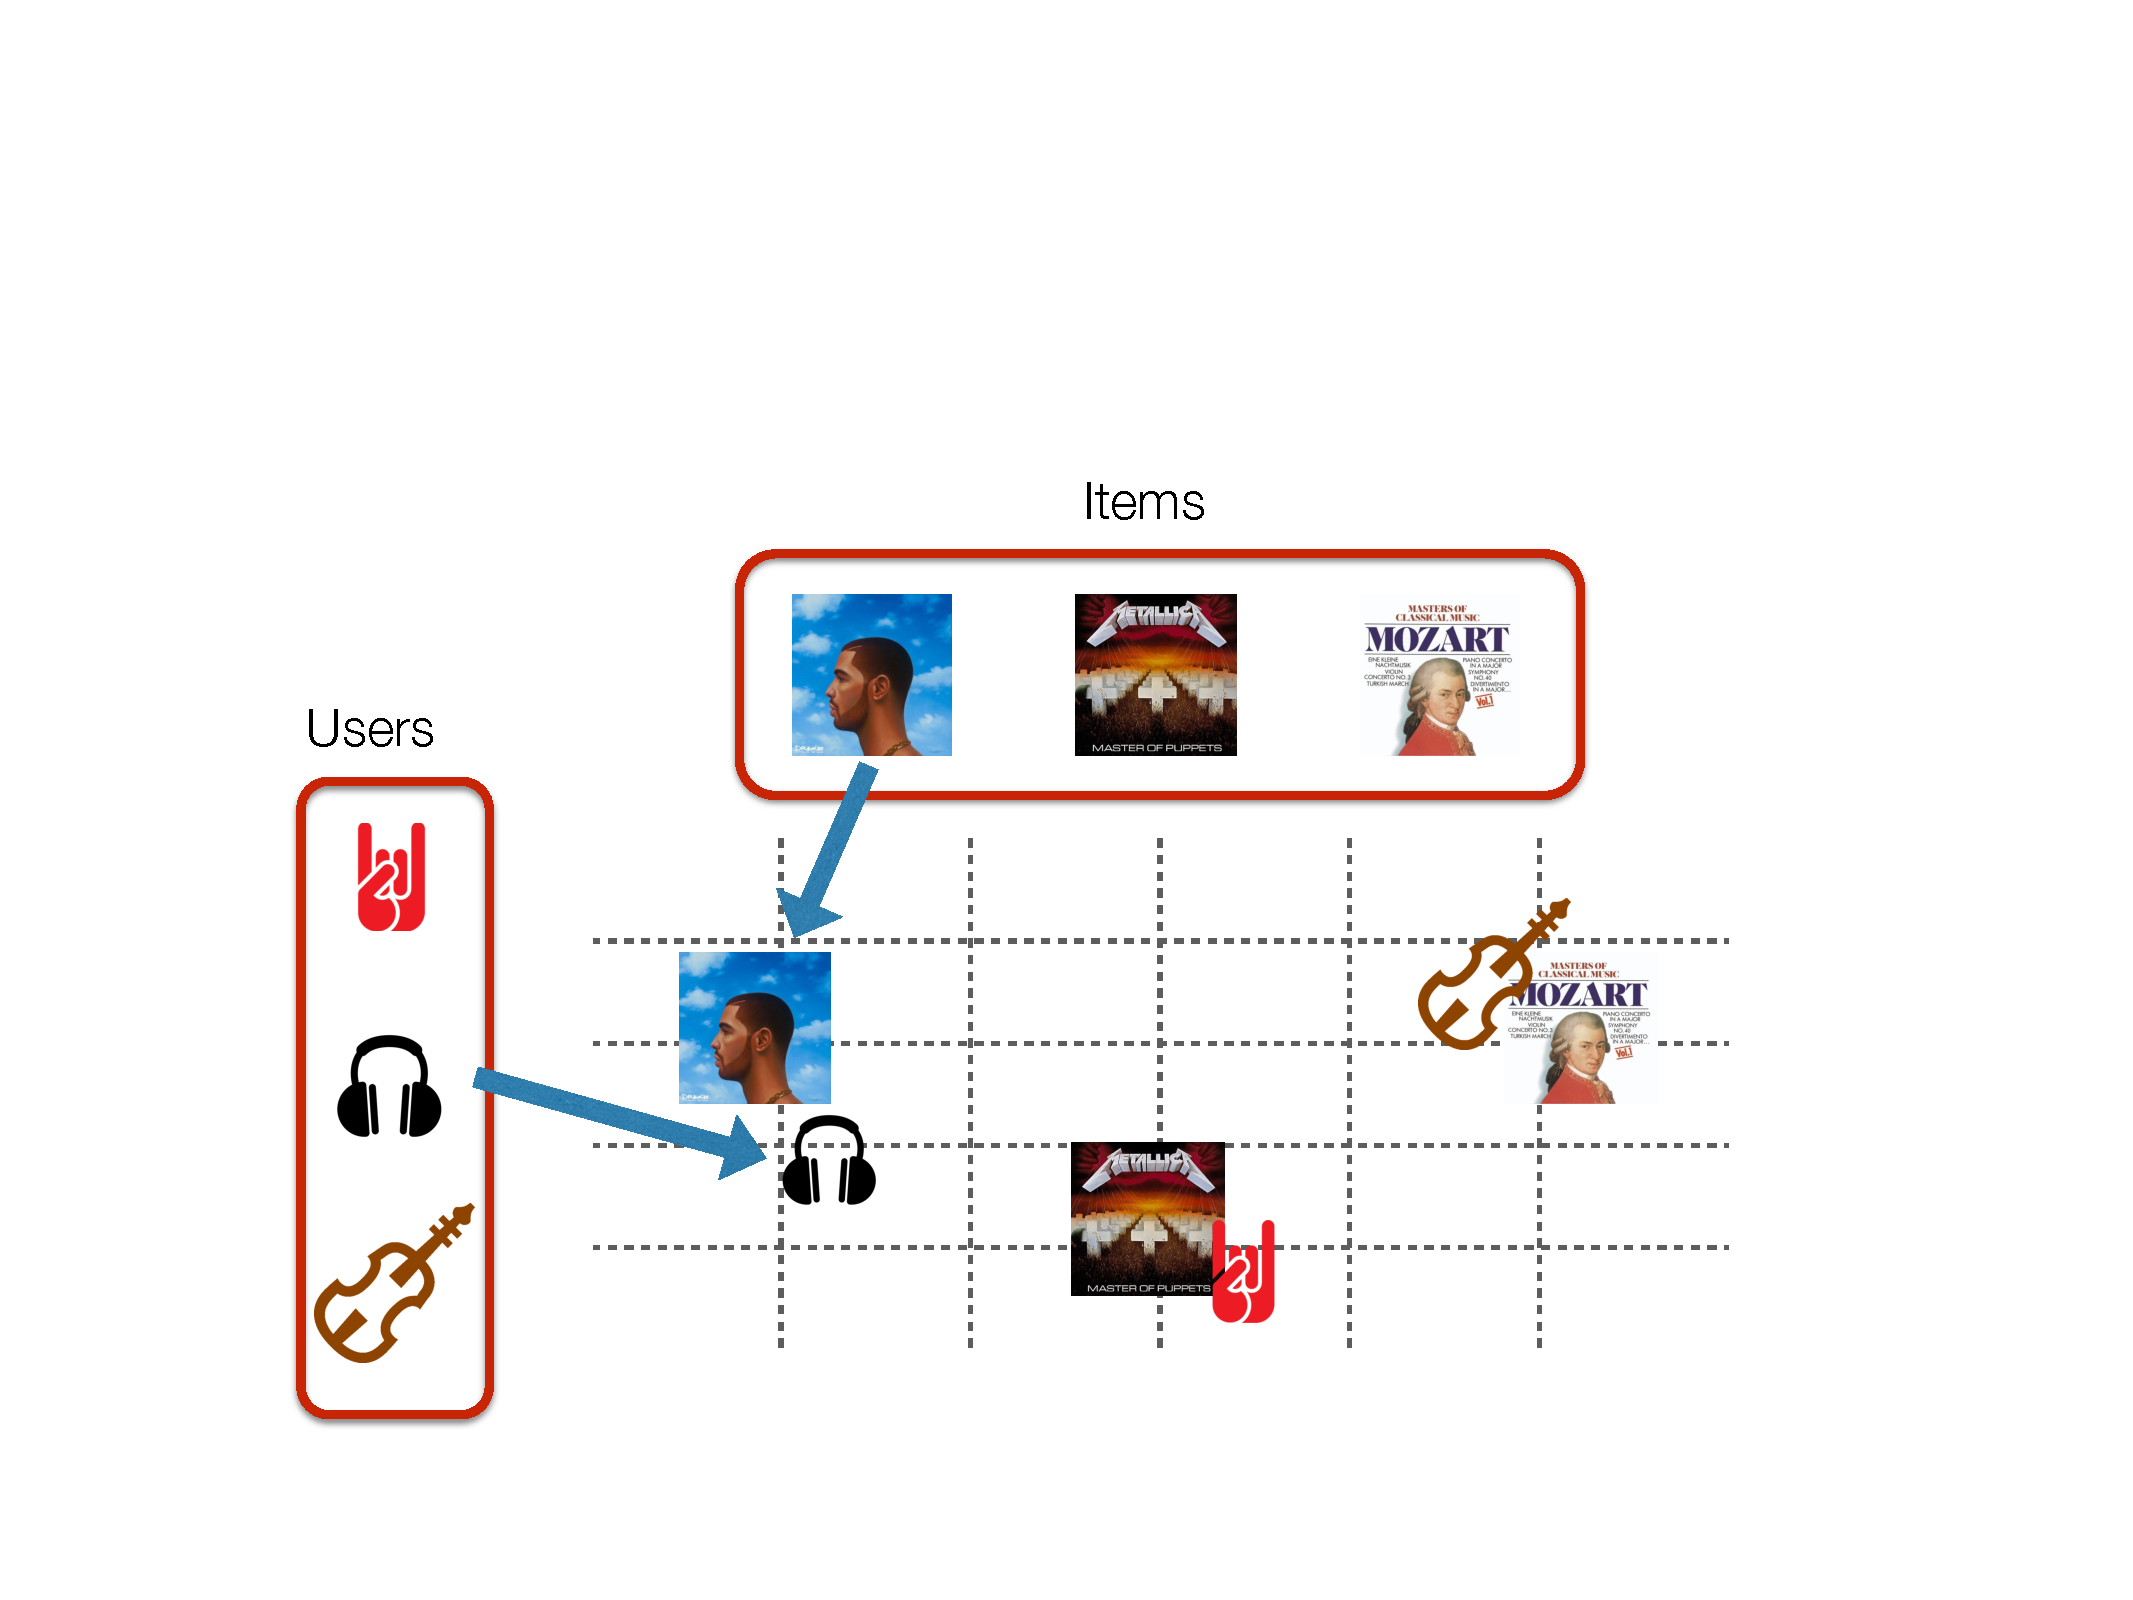
\includegraphics[width=\textwidth]{fig/cf_cartoon}
      \caption{An illustrative example of matrix factorization for collaborative filtering. Matrix factorization aims to find a latent preference space to embed both users and items such that if a user consumes an item, they will be embedded closer in this latent space.}
      \label{chpt:background:fig:cf_cartoon}
\end{figure}

\Cref{chpt:background:fig:cf_cartoon} demonstrates the basic idea behind matrix factorization for collaborative filtering.\footnote{This figure is only an illustrative example: typical matrix factorization models use inner products, not Euclidean distance, to measure similarity.} In this illustrative example, we have three users and three items, where each user consumes only one item. Matrix factorization aims to find a latent space to embed all of the users and items. If a user consumes an item, this user and item pair will be embedded closer in this latent space. The locations (coordinates) in this latent space correspond to the user and item latent factors obtained by factorizing the click matrix. To make recommendations for each user, we select the unconsumed items which have high dot products with the user's latent factor. 

How would this work? Consider a metalhead who has listened to a lot of \textit{Metallica} but not \textit{Iron Maiden}. It is reasonable to assume that there are many other users with similar tastes listened to songs from both bands, which makes the latent factors for songs by both \textit{Metallica} and \textit{Iron Maiden} very close in the latent space. Therefore, when making recommendations for this user, the songs from \textit{Iron Maiden} will likely have higher dot products, which will be recommended by the learned matrix factorization model.  

From a generative modeling perspective, the model can be understood as first drawing user and item latent factors corresponding,
respectively, to user preferences and item attributes. Then drawing 
observations from a specific distribution (e.g., a Poisson
or a Gaussian) with its mean parametrized by the dot product between the user and
the item factors. Formally, Gaussian matrix factorization is \citep{salakhutdinov2008probabilistic}: 
\begin{equation} 
\begin{split}
	\mb\theta_{u} &\sim \mathcal{N}(\bzero, \lambda_\theta^{-1} \mathrm{I}_K) \quad \textrm{for } u = 1, \dots, U, \\
	\mb\beta_{i} &\sim \mathcal{N}(\bzero, \lambda_\beta^{-1} \mathrm{I}_K) \quad \textrm{for } i = 1, \dots, I, \\
	y_{ui} &\sim \mathcal{N}(\mb\theta_u^\top \mb\beta_i, \lambda_y^{-1}) \quad \textrm{for } (u, i) \in \cO, 
 \end{split}
 \label{chpt:background:eq:gmf}
 \end{equation}
where $\mb\theta_u$ and $\mb\beta_i$ represent user $u$'s latent preferences and item $i$'s attributes respectively. We use the mean and (co)variance to
parametrize the Gaussian distribution. $\lambda_\theta$, $\lambda_\beta$, and
$\lambda_y$ can be treated as hyperparameters, or be given priors for a full Bayesian treatment. $\mathrm{I}_K$ stands for the identity
matrix of dimension $K$. A graphical model representation of the Gaussian matrix factorization model is shown in \Cref{chpt:background:fig:gmf}.

\begin{figure}[ht]
  \centering
     \begin{tikzpicture}

 % Define nodes
  \node[obs]                               (y) {$y_{ui}$};
  \node[latent, above=of y, xshift=-1.2cm] (w) {$\mb\theta_u$};
  \node[latent, above=of y, xshift=1.2cm]  (x) {$\mb\beta_i$};
  \node[const, right=2cm of y]            (t) {$\lambda_y$};
  \node[const, above=of w] (lw) {$\lambda_\theta$};
  \node[const, above=of x] (lx) {$\lambda_\beta$};


  % Connect the nodes
  \edge {x,w,t} {y} ; %
  \edge {lw} {w};
  \edge {lx} {x};

  % Plates
  \plate {yx} {(x)(y)} {$I$} ;
  \plate {} {(w)(y)(yx.north west)(yx.south west)} {$U$} ;

\end{tikzpicture}

  \caption{Graphical model representation for the Gaussian matrix factorization.}
\label{chpt:background:fig:gmf}
\end{figure}

We derive coordinate updates to obtain the maximum \textit{a posteriori} estimates of the Gaussian matrix factorization model, as they are closely related to the model inference we develop in the later chapters. Since we are only obtaining point estimates of the model parameters, we can always scale $\lambda_\theta$ and $\lambda_\beta$ by $\lambda_y$ to obtain the same solution. Without loss of generality, we set $\lambda_y = 1$. The complete log-likelihood of the model is:

\begin{equation}
\cL = -\sum_{(u, i)\in \cO} \frac{1}{2}(y_{ui} - \mb\theta_u^\top\mb\beta_i)^2 - \frac{\lambda_\theta}{2} \sum_u \|\mb\theta_u \|^2_2 - \frac{\lambda_\beta}{2} \sum_i \|\mb\beta_i \|_2^2.
\label{chpt:background:eq:gmf_logll}
\end{equation}

As we can see, the maximum \emph{a posteriori} estimates of the Gaussian matrix factorization model is equivalent to the solution of minimizing the squared loss between the estimated and actual preferences $\sum_{(u, i)\in \mathcal{O}} (y_{ui} - \mb\theta_u^\top\mb\beta_i)^2$ with $\ell_2$ regularization on the latent factors.

The basic idea of the coordinate updates for the Gaussian matrix factorization model is to only update one of the user or item factor ($\mb\theta_u$ or $\mb\beta_i$) at a time when keeping everything else fixed. Taking the gradient of the complete log-likelihood (\Cref{chpt:background:eq:gmf_logll}) with respect to one of the latent factors and setting it to $0$, we obtain the following updates:

\begin{equation}
\mb\theta_u^\new \leftarrow (\sum_{i: (u, i) \in \cO} \mb\beta_i \mb\beta_i^\top + \lambda_\theta \mathrm{I}_K)^{-1} (\sum_{i: (u, i) \in \cO} y_{ui} \mb\beta_i)
\label{chpt:background:eq:als_user}
\end{equation}
\begin{equation}
\mb\beta_i^\new \leftarrow (\sum_{u: (u, i)\in\cO} \mb\theta_u \mb\theta_u^\top + \lambda_\beta \mathrm{I}_K)^{-1} (\sum_{u: (u, i)\in\cO} y_{ui} \mb\theta_u)
\label{chpt:background:eq:als_item}
\end{equation}

Every single update resembles that of ridge regression \citep{friedman2001elements} where the responses are $y_{ui}$ and the covariates are the latent factors. Therefore, the coordinate updates for the Gaussian matrix factorization is often called \textit{alternating least squares} (ALS). The full algorithm is summarized in \Cref{chpt:background:algo:gmf}. Note that the updates are embarrassingly parallelizable across users and items. 

\begin{algorithm}
\DontPrintSemicolon % Some LaTeX compilers require you to use \dontprintsemicolon instead 
\KwIn{A set of observed entires in the click matrix $\{y_{ui}: (u, i)\in\cO\}$, regularization parameters $\lambda_\theta$ and $\lambda_\beta$}
\KwOut{A set of user latent factors $\mb\theta_{1:U}$ and item latent factors $\mb\beta_{1:I}$}
%$C \gets \emptyset$\;
Randomly initialize $\mb\theta_{1:U}$, $\mb\beta_{1:I}$\;
\While{not converged}{
  \For{$u \gets 1$ \textbf{to} $U$}{
  	Update user factor $\mb\theta_u$ (\Cref{chpt:background:eq:als_user})
	}
  \For{$i \gets 1$ \textbf{to} $I$}{
  	Update item factor $\mb\beta_i$  (\Cref{chpt:background:eq:als_item})
	}
}
\Return{$\mb\theta_{1:U}$, $\mb\beta_{1:I}$}\;
\caption{{\sc ALS} Alternating least squares for the Gaussian matrix factorization}
\label{chpt:background:algo:gmf}
\end{algorithm}

\subsubsection{Collaborative filtering for implicit data} 
\label{chpt:background:sec:cf_implicit}

The model described in \Cref{chpt:background:eq:gmf} can be equally applied to both explicit and implicit data. The real difference is how to define the observed set $\cO$: For explicit data, it can simply be the user-item pairs where user $u$ has clicked on (rated) item $i$. However, we can not copy the same definition for implicit data. The reason is that the data is binary and thus, when inferring a user's preferences, we must use unclicked items (otherwise, it would be like training a classifier with only positive labels\footnote{Recommendation from implicit data is also known as one-class collaborative filtering \citep{pan2008one}.}), i.e., $\cO$ contains all the entires in the click matrix. 

Mirroring methods for explicit data, many methods treat unclicked items as those a user does not like.  But this assumption is mistaken, and overestimates the effect of the unclicked items.  Some of these
items---many of them, in large-scale settings---are unclicked because
the user didn't see them, rather than because she chose not to
click them.  This is the crux of the problem of analyzing implicit
data: we know users click on items they like, but we do not know why
an item is unclicked.
	
\gls{WMF}, the standard factorization model for implicit
data, selectively downweights evidence from the click
matrix~\citep{hu2008collaborative}.  \gls{WMF} uses a simple heuristic where all
unobserved user-item interactions are equally downweighted vis-a-vis the
observed interactions. Under \gls{WMF} an observation is generated from:
\begin{align*} 
y_{ui} &\sim \mathcal{N}(\mb\theta_u^\top\mb\beta_i, c^{-1}_{y_{ui}}),
\end{align*}
where the ``confidence'' $c$ is set such that $c_1 > c_0$. This dependency between a
click and itself is unorthodox; because of it \gls{WMF} is not a generative
model. As we will describe in \Cref{chpt:expomf} we obtain a proper generative
model by adding an exposure latent variable. 

The maximum \textit{a posteriori} estimates of \gls{WMF} can also be obtained via ALS with minor modification. For notational convenience, we define $c_{ui} \triangleq c_{y_{ui}}$. The complete log-likelihood for \gls{WMF} is (recall that observed set $\cO$ contains all the entries in the click matrix):
\begin{equation*}
\cL = -\sum_{u, i} \frac{c_{ui}}{2}(y_{ui} - \mb\theta_u^\top\mb\beta_i)^2 - \frac{\lambda_\theta}{2} \sum_u \|\mb\theta_u \|^2_2 - \frac{\lambda_\beta}{2} \sum_i \|\mb\beta_i \|_2^2
\end{equation*}
Again, we take the gradient with respect to one of the factors and set it to $0$, which leads to the following ALS updates:
\begin{equation}
\mb\theta_u^\new \leftarrow (\sum_i c_{ui} \mb\beta_i \mb\beta_i^\top + \lambda_\theta \mathrm{I}_K)^{-1} (\sum_i c_{ui} y_{ui} \mb\beta_i)
\label{chpt:background:eq:wals_user}
\end{equation}
\begin{equation}
\mb\beta_i^\new \leftarrow (\sum_u c_{ui} \mb\theta_u \mb\theta_u^\top + \lambda_\beta \mathrm{I}_K)^{-1} (\sum_u c_{ui} y_{ui} \mb\theta_u)
\label{chpt:background:eq:wals_item}
\end{equation}

However, unlike \Cref{chpt:background:eq:als_user} and \Cref{chpt:background:eq:als_item}, the summation inside of the matrix inversion is over all the users or items, which can be computationally challenging, especially considering that we will have to do this computation for every single factor update (there are in total $U + I$ factors to be updated in one iteration). \citet{hu2008collaborative} propose a clever trick to speed up the computation substantially by breaking up the summation into two parts as follows (here we only demonstrate the case for updating the user factor $\mb\theta_u$, the same can be applied to item factor $\mb\beta_i$):
\begin{align*}
&(\sum_i c_{ui} \mb\beta_i \mb\beta_i^\top + \lambda_\theta \mathrm{I}_K)^{-1} (\sum_i c_{ui} y_{ui} \mb\beta_i)\\
=~& (\sum_i (c_{ui} - c_0) \mb\beta_i \mb\beta_i^\top + \underbrace{\sum_i c_0 \mb\beta_i \mb\beta_i^\top + \lambda_\theta \mathrm{I}_K}_{\textrm{precompute once per iteration}})^{-1} (\sum_i c_{ui} y_{ui} \mb\beta_i).
\end{align*}

The second part $\sum_i c_0 \mb\beta_i \mb\beta_i^\top + \lambda_\theta \mathrm{I}_K$ is shared across all the user factor updates, thus can be precomputed once per iteration. The first part $\sum_i (c_{ui} - c_0)\mb\beta_i\mb\beta_i^\top$ can be efficiently computed because $c_{ui} - c_0$ is non-zero only when $y_{ui} = 1$ and normally the click matrix is highly sparse. Furthermore, just like ALS for the Gaussian matrix factorization, all the updates are embarrassingly parallelizable across users and items. The full algorithm of ALS for \gls{WMF} is summarized in \Cref{chpt:background:algo:wmf}. With the speed-up trick and embarrassing parallelization, ALS for \gls{WMF} can be easily applied to datasets with millions of users and items. 

\begin{algorithm}
\DontPrintSemicolon % Some LaTeX compilers require you to use \dontprintsemicolon instead 
\KwIn{Click matrix $y_{ui}$, the confidence for clicked $c_1$ and unclicked $c_0$, regularization parameters $\lambda_\theta$ and $\lambda_\beta$}
\KwOut{A set of user latent factors $\mb\theta_{1:U}$ and item latent factors $\mb\beta_{1:I}$}
%$C \gets \emptyset$\;
Randomly initialize $\mb\theta_{1:U}$, $\mb\beta_{1:I}$\;
\While{not converged}{
  Precompute $\sum_i c_0 \mb\beta_i \mb\beta_i^\top + \lambda_\theta \mathrm{I}_K$\;
  \For{$u \gets 1$ \textbf{to} $U$}{
  	Update user factor $\mb\theta_u$ (\Cref{chpt:background:eq:wals_user})
	}
  Precompute $\sum_u c_0 \mb\theta_u \mb\theta_u^\top + \lambda_\beta \mathrm{I}_K$\;
  \For{$i \gets 1$ \textbf{to} $I$}{
  	Update item factor $\mb\beta_i$  (\Cref{chpt:background:eq:wals_item})
	}
}
\Return{$\mb\theta_{1:U}$, $\mb\beta_{1:I}$}\;
\caption{{\sc W-ALS} Alternating least squares for \gls{WMF}}
\label{chpt:background:algo:wmf}
\end{algorithm}

\gls{WMF} treats the collaborative filtering problem with implicit data as a
regression problem. Concretely, consumed user-item pairs are assigned a
value of one and unobserved user-item pairs are assigned a value of zero.
Bayesian personalized ranking (BPR) \citep{rendle2009bpr,
rendle2014improving} instead treats the problem as a one of ranking
consumed user-item pairs above unobserved pairs.
In a similar vein, the weighted approximate-ranking pairwise (WARP) loss
proposed in \citet{weston2011wsabie} approximately optimizes Precision@$k$. 
To deal with the non-differentiable nature of the ranking
loss, these methods typically design specific (stochastic optimization)
methods for parameter estimation.

%with closed-form
%model inference, these methods typically require specifically designed
%stochastic method for parameter estimation.   

\section{Causal inference}\label{chpt:background:sec:causal}

Causal inference is aiming to answer the cause-and-effect question: does $X$ cause $Y$? If so, how much is the effect of $X$ on $Y$? Causal inference helps us learn about how things work and predict what happens when certain things change \citep{morgan2014counterfactuals,imbens2015causal}. 
%We are not particularly interested in asking such \textit{counterfactual} question about recommendation. Instead, we formulate recommendation as performing model inference from (biased) observational data and use the tools developed in causal inference to help us make better prediction about users' future preference. 
In this section, we review some basic concepts of causal inference that will be used in the later chapters of this dissertation when we make a connection between causal inference and recommendation.  

\subsection{Potential outcome framework}\label{chpt:background:sec:potential}

The potential outcome framework of causal inference \citep{rubin1974ece} is the most widely used causality formulation. We use random variable $A = a$ as an indicator of treatment assignment and assume the treatment is binary, i.e., $a$ is either $1$ (assigned the treatment) or $0$ (not assigned the treatment). In this framework, each individual has two \textit{potential outcomes} $Y(a)$ depending on the value of $a$. For example, in a medical trial, for each patient, we assume there is a potential outcome $Y(1)$ if she receives the treatment and $Y(0)$ if she receives the placebo. 

One measurement of the causal effect is the average difference (over individuals) between those potential outcomes. It is formally formulated as the \gls{ATE}: $\E{\delta} = \E{Y(1)} - \E{Y(0)}$, where the expectation is taken over the whole population of interest. In the language of graphical models \citep{pearl2009causality},
this is framed as evaluating the impact of an intervention on random variables in a probabilistic graph. The difficulty of causal inference is that we can only observe one realization of all the potential outcomes $Y(a)$, for $a\in\{0, 1\}$. 

\subsection{Randomized experiments and observational studies} \label{chpt:background:sec:exp_obs}

% \PP Under the assumption of unconfoundednessm, strong ignorability:
% \begin{equation*}
% Y(0), Y(1) \indpt A \g x
% \end{equation*}
% we can obtain an unbiased estimate of the \gls{ATE}.

There are two types of data commonly encountered in causal analysis: data collected from randomized experiments and data collected from observational studies. 

Randomized experiments are the experiments that each unit receives treatment randomly (e.g., a medical trial where a random proportion of patients receives treatment). They allow the great reliability and validity of statistical estimates of causal effects. A naive \gls{ATE} estimator of the difference between the treated and untreated with data from randomized experiments is unbiased. Such data is of great quality, but sometimes it is impossible to obtain. 

Observational data, on the other hand, is collected from an observational study where we have no control over the assignment mechanism. This can happen when it is impractical to perform a randomized experiment (e.g., for ethical reasons) or when we cannot control the data collecting process. Special care is required when making causal statement with observational data, since the naive \gls{ATE} estimator is generally biased. Despite such difficulty, observational data is easily accessible comparing to data collected from randomized experiments.

If we treat recommending an item to a user as assigning a treatment, the data collected from a typical recommender system is an example of observational data. We leverage this connection in \Cref{chpt:causal_rec} to develop a causal inference approach to recommendation. 





